% === Revised Section 6: AIXI ===
%
% NEW PREAMBLE ADDITIONS NEEDED:
% \usepackage{tikz}
% \usetikzlibrary{trees, positioning, arrows.meta}
% \usepackage{listings}
% \lstset{basicstyle=\ttfamily\footnotesize, frame=single, breaklines=true,
%         columns=fullflexible, keepspaces=true}
%
% \newtcolorbox{activity}[1][]{
%   breakable, enhanced,
%   colback=blue!4, colframe=blue!55!black,
%   coltitle=white, fonttitle=\bfseries,
%   title={Activity}, boxrule=0.6pt,
%   left=6pt,right=6pt,top=4pt,bottom=4pt,
%   #1
% }
%
% (The \texttt{intuition} and \texttt{example} environments already exist in
% the document preamble --- see lines 26--49.)

\section{AIXI: intelligence as optimal compression-driven prediction}
\label{sec:aixi}
% =========================================================================

\begin{intuition}
\textbf{One-line version.}  AIXI is the agent that, before every move,
asks every possible theory of the world ``what happens if I do this?'',
weights each theory by how short it is, averages the predicted rewards,
and picks the action with the highest weighted total
(\cref{def:aixi,thm:aixi-opt}).  It is a \emph{definition of optimal
behaviour}, not a product --- the averaging step requires infinite
compute.

\textbf{The regional-manager analogy.}  Imagine a regional manager who,
before every staffing decision, consulted every possible theory of her
stores --- every demand model, every weather-effect hypothesis, every
crank manifesto about Mercury retrograde --- weighted by how simple
each theory is.  For each candidate decision she asks: ``If I do this,
what happens over the next hundred Tuesdays, and how much will I enjoy
it?''  She takes the weighted average and places the staffing bet that
maximises expected sales across all of them.  That manager would be
provably optimal in a precise technical sense.  She would also be
impossible: consulting every possible theory takes infinite time.
This is AIXI.

\textbf{Or, the auditor story.}  AIXI is the diligent auditor who,
before approving a single expense report, reads every audit manual
ever written in every language, ranks them by length, and adjudicates
the expense by simplicity-weighted consensus.  The auditor is never
wrong in principle.  The auditor also never approves anything.  Real
audit teams are food trucks reading the Michelin menu; AIXI is the
chef with an infinite pantry and no kitchen.

\textbf{Why compression is the whole story.}  AIXI's only prior is
Occam's razor: short theories get exponentially more weight than long
ones.  That single ingredient --- plus bookkeeping --- is enough to
produce universally optimal action.  Intelligence, in this framework,
\emph{is} compression plus planning.

\textbf{The catch.}  AIXI is uncomputable; it requires running every
possible program.  Bounded approximations exist but are toys at
present.  AIXI is to intelligence what the ideal gas law is to a real
gas --- a north star, not a product.

\textbf{Why a decision-maker should care.}  AIXI is a crisp,
non-hand-wavy definition of ``what would a perfectly general AI do?''
When someone claims their system is ``a step toward AGI,'' ask: is it
a step toward better approximating AIXI?  Is it building better
world-models (compression) and planning against them (expectimax)?  If
yes, the claim is in the right ballpark.  If it is pattern-matching in
a narrow domain with no planning layer, the claim is marketing.  No
real system \emph{is} AIXI, so any product advertised as ``universal
intelligence'' is abusing the term.
\end{intuition}

\subsection*{From passive prediction to sequential action}

Hutter's AIXI framework \citep{hutter2005universal} extends Solomonoff
induction from passive sequence prediction to sequential
decision-making.  Where Solomonoff's agent only had to \emph{predict}
the next bit, AIXI has to \emph{act} and then see what the environment
does back.

The setup.  The agent interacts with an environment over discrete time
steps.  At step $t$ the agent chooses an action $a_t \in
\mathcal{A}_{\mathrm{act}}$, and the environment returns a
\emph{percept} $e_t = (o_t, r_t)$ consisting of an observation $o_t
\in \mathcal{O}$ (``what I see'') and a reward $r_t \in [0,
r_{\max}]\subset\mathbb{R}$ (``how much I liked it'').  Write the
interaction history as
\[
  h_{<t} \;=\; (a_1, e_1, a_2, e_2, \dots, a_{t-1}, e_{t-1}).
\]
Think of $h_{<t}$ as the manager's logbook so far.

An \textbf{environment} $\nu$ is a conditional probability measure
$\nu(e_{1:m}\mid a_{1:m})$: given the agent's planned action sequence,
it tells you how likely any percept sequence is.  An environment is
the ``true world''; the agent does not know which one it is in.

The \textbf{universal mixture environment} $\xi$ is the
Solomonoff-style weighted average over all of them:
\begin{equation}
  \xi(e_{1:m} \mid a_{1:m})
  \;=\; \sum_{\nu \in \mathcal{M}} 2^{-K(\nu)}\;\nu(e_{1:m} \mid a_{1:m}),
  \label{eq:xi}
\end{equation}
where $\mathcal{M}$ is the class of all lower-semicomputable
(``chronological'') environments and $K(\nu)$ is the Kolmogorov
complexity of a prefix program for $\nu$.  The weight $2^{-K(\nu)}$ is
Occam's razor made numerical: halving the description length
\emph{squares} the weight.

\begin{intuition}
Read \eqref{eq:xi} like this: ``the probability my mixture assigns to
seeing percepts $e_{1:m}$ after actions $a_{1:m}$ is a
simplicity-weighted vote among every computable theory of the world.''
The vote never converges to one theory unless that theory is the only
short one compatible with the data.
\end{intuition}

\subsection*{The AIXI action rule}

\begin{definition}[AIXI]
\label{def:aixi}
Fix a finite planning horizon $m$ and (optionally) a discount factor.
The \textbf{AIXI action} at history $h_{<t}$ is
\begin{equation}
  a_t^{\mathrm{AIXI}}
  \;=\; \arg\max_{a_t}
        \sum_{e_t}\!\max_{a_{t+1}}\sum_{e_{t+1}}\!\cdots\!\max_{a_m}\sum_{e_m}
        \Bigl(\sum_{k=t}^{m} r_k\Bigr)\,
        \xi\bigl(e_{t:m}\,\big|\,h_{<t}, a_{t:m}\bigr).
  \label{eq:aixi-rule}
\end{equation}
Each $\max_{a_\tau}$ says ``pick the best action I could possibly take
at step $\tau$''; each $\sum_{e_\tau}$ says ``average over what the
environment might show me, weighted by the universal mixture $\xi$.''
The inner $\sum_{k=t}^{m} r_k$ is the total reward collected along a
given rollout.
\end{definition}

\paragraph{In words.}  AIXI plans by \emph{expectimax} over all
possible futures, where ``possible'' is weighted by the universal
mixture~\eqref{eq:xi}.  The $2^{-K(\nu)}$ weighting is what ties the
definition of intelligence back to compression: hypothesised
environments with short descriptions receive exponentially more
weight.  An AIXI-optimal agent simultaneously (i) compresses its
environment optimally and (ii) acts to maximise reward under that
compressed model.

\subsection*{Drawing the expectimax tree}

Nested $\max$-$\sum$ notation is easy to write and hard to read.
\Cref{fig:expectimax} is the same equation as \eqref{eq:aixi-rule},
drawn for $2$ actions, $2$ percepts, and $2$ plies of lookahead.

\begin{figure}[h]
\centering
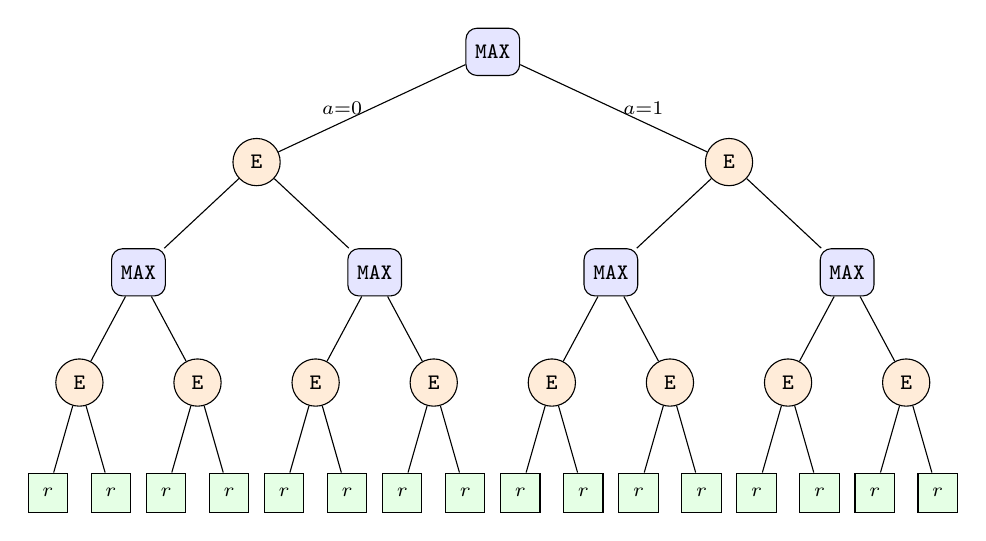
\begin{tikzpicture}[
  level distance=14mm,
  level 1/.style={sibling distance=60mm},
  level 2/.style={sibling distance=30mm},
  level 3/.style={sibling distance=15mm},
  level 4/.style={sibling distance=8mm},
  act/.style ={draw, rectangle, rounded corners, fill=blue!10, minimum size=6mm, font=\footnotesize},
  perc/.style={draw, circle, fill=orange!15, minimum size=6mm, font=\footnotesize},
  leaf/.style={draw, rectangle, fill=green!10, minimum size=5mm, font=\scriptsize},
  every node/.style={font=\footnotesize},
]
\node[act] (root) {\texttt{MAX}}
  child {node[perc] {\texttt{E}}
    child {node[act] {\texttt{MAX}}
      child {node[perc] {\texttt{E}}
        child {node[leaf] {$r$}}
        child {node[leaf] {$r$}}}
      child {node[perc] {\texttt{E}}
        child {node[leaf] {$r$}}
        child {node[leaf] {$r$}}}}
    child {node[act] {\texttt{MAX}}
      child {node[perc] {\texttt{E}}
        child {node[leaf] {$r$}}
        child {node[leaf] {$r$}}}
      child {node[perc] {\texttt{E}}
        child {node[leaf] {$r$}}
        child {node[leaf] {$r$}}}}
    edge from parent node[left, font=\scriptsize] {$a{=}0$}}
  child {node[perc] {\texttt{E}}
    child {node[act] {\texttt{MAX}}
      child {node[perc] {\texttt{E}}
        child {node[leaf] {$r$}}
        child {node[leaf] {$r$}}}
      child {node[perc] {\texttt{E}}
        child {node[leaf] {$r$}}
        child {node[leaf] {$r$}}}}
    child {node[act] {\texttt{MAX}}
      child {node[perc] {\texttt{E}}
        child {node[leaf] {$r$}}
        child {node[leaf] {$r$}}}
      child {node[perc] {\texttt{E}}
        child {node[leaf] {$r$}}
        child {node[leaf] {$r$}}}}
    edge from parent node[right, font=\scriptsize] {$a{=}1$}};
\end{tikzpicture}
\caption{Expectimax tree behind \eqref{eq:aixi-rule}, drawn for two
actions, two possible percepts, and two plies.  Blue squares are
\texttt{MAX} (agent chooses); orange circles are \texttt{E} (weighted
average under $\xi$); green leaves hold a cumulative reward.  AIXI is
exactly this tree, but (i) infinitely wide in branching, (ii)
infinitely deep, and (iii) with each orange \texttt{E} node averaging
over \emph{every computable theory} of the world.}
\label{fig:expectimax}
\end{figure}

\subsection*{A 2-hypothesis worked example}

We now collapse \eqref{eq:aixi-rule} to arithmetic on a toy world.

\begin{example}[Two-step, two-hypothesis AIXI]
\label{ex:aixi-hand}
Actions $\mathcal{A}_{\mathrm{act}}=\{A,B\}$, percepts $\{0,1\}$ (with
$r_t = e_t$: a percept $1$ gives reward $1$).  Horizon $m=2$.  Suppose
the mixture has collapsed to just two live hypotheses with posterior
weights
\[
  w_{\mathrm{simple}}=\tfrac{3}{4},\qquad w_{\mathrm{complex}}=\tfrac{1}{4}.
\]
\textbf{Simple theory:} ``$A$ pays $1$ w.p.\ $0.6$; $B$ pays $1$ w.p.\
$0.3$; independent of history.''
\textbf{Complex theory:} ``$A$ pays $1$ w.p.\ $0.3$; $B$ pays $1$ w.p.\
$0.8$; independent of history.''

For the one-step case (ignore second step), the expected immediate
reward of pulling $A$ is
\[
  \mathbb{E}_\xi[r \mid A]
  \;=\; \tfrac{3}{4}\cdot 0.6 + \tfrac{1}{4}\cdot 0.3
  \;=\; 0.525,
\]
and of pulling $B$ is
\[
  \mathbb{E}_\xi[r \mid B]
  \;=\; \tfrac{3}{4}\cdot 0.3 + \tfrac{1}{4}\cdot 0.8
  \;=\; 0.425.
\]
AIXI picks $A$.  Note the complex theory is kept alive --- it still
gets $25\%$ of the vote --- which is why a future observation of $B$
paying out would swing the posterior fast.  \emph{Exploration is not
programmed in; it is a side effect of keeping every theory on the
books.}

For the full two-step case, the student repeats the same arithmetic
inside each branch of \cref{fig:expectimax}.  The horizon-$2$ answer
is still $A$ first, and the reader should verify it on the worksheet
below.
\end{example}

\subsection*{Universal optimality}

\begin{theorem}[Universal optimality of AIXI, informal]
\label{thm:aixi-opt}
Within the class of lower-semicomputable environments, AIXI is
\emph{Pareto optimal}: no agent $\pi'$ achieves strictly greater
expected total reward than AIXI in \emph{every} environment $\nu \in
\mathcal{M}$.  Moreover, for any computable $\nu$ the AIXI predictor
converges to the true environment's predictions in the sense of
\eqref{eq:sol-bound} with $M$ replaced by~$\xi$.
\end{theorem}

\begin{intuition}
Pareto-optimal is a \emph{weak} optimality guarantee and it is
important to be honest about it.  It says: no rival agent strictly
dominates AIXI across all worlds.  It does \emph{not} say AIXI is best
on average in the world you actually live in.  A specialist agent
handcrafted for chess will beat AIXI at chess; it will just lose to
AIXI on the average of all computable games.  Picture a
Pareto frontier (\cref{fig:pareto}): AIXI sits on the frontier, but so
do many narrower agents.  The content of \cref{thm:aixi-opt} is
``AIXI is not dominated,'' not ``AIXI is uniquely best.''
\end{intuition}

\begin{figure}[h]
\centering
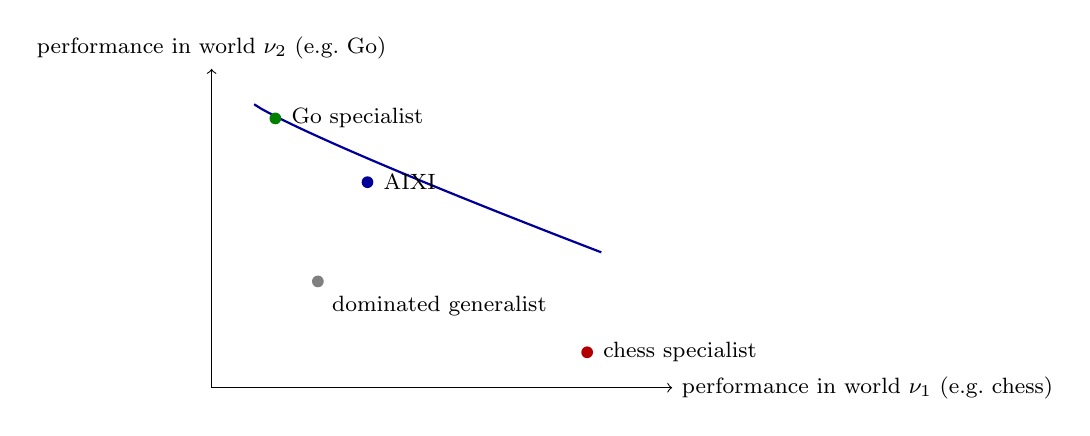
\begin{tikzpicture}[scale=0.9]
  \draw[->] (0,0) -- (6.5,0) node[right] {\footnotesize performance in world $\nu_1$ (e.g.\ chess)};
  \draw[->] (0,0) -- (0,4.5) node[above] {\footnotesize performance in world $\nu_2$ (e.g.\ Go)};
  \draw[thick, blue!60!black, domain=0.6:5.5, samples=50]
       plot (\x, {4 - 0.5*(\x-0.6)^0.9});
  \node[circle, fill=blue!60!black, inner sep=1.5pt, label={right:\footnotesize AIXI}] at (2.2, 2.9) {};
  \node[circle, fill=red!70!black,  inner sep=1.5pt, label={right:\footnotesize chess specialist}] at (5.3, 0.5) {};
  \node[circle, fill=green!50!black,inner sep=1.5pt, label={right:\footnotesize Go specialist}] at (0.9, 3.8) {};
  \node[circle, fill=gray,          inner sep=1.5pt, label={below right:\footnotesize dominated generalist}] at (1.5, 1.5) {};
\end{tikzpicture}
\caption{Cartoon Pareto frontier across two environments.  AIXI lies
on the frontier (no agent strictly dominates it), and so do the narrow
specialists.  Only the grey ``dominated generalist'' is strictly
worse than something else in both worlds.}
\label{fig:pareto}
\end{figure}

For the precise statement and proof see
\citet[Ch.~5]{hutter2005universal}.  The significance of
\cref{thm:aixi-opt} is that ``intelligence'' has, within this
framework, been reduced to a single ingredient (the universal
prior~\eqref{eq:xi}) plus bookkeeping (the expectimax expansion).
Remove the Solomonoff prior and the agent collapses to uninformed
search; keep it, and the agent becomes universally optimal in the
Pareto sense.

\subsection*{Activities}

\begin{activity}[title={Activity A: Two-armed bandit, live in the room}]
\textbf{Goal.}  Feel in your bones why simplicity-weighting produces
exploration for free.

\textbf{Setup.}  Pair up.  One partner is the \emph{environment}: they
secretly fix probabilities $(p_A, p_B)\in[0,1]^2$ for arms $A$ and $B$
paying out, and flip accordingly.  The other partner is the
\emph{agent} and plays $20$ rounds.  The agent carries two paper
advisors: a \emph{simple advisor} who insists on the current
empirical-best arm, and a \emph{complex advisor} who insists the other
arm is due.  At each round the agent rolls a die to weight the two
advisors $\tfrac{3}{4} : \tfrac{1}{4}$ and plays their weighted vote.

\textbf{Debrief.}  Count total reward.  Compare to a ``greedy'' agent
who always pulls the empirical-best arm.  Discuss: where did the
simplicity-weighting kick in?  When did the complex advisor save the
day?
\end{activity}

\begin{activity}[title={Activity B: Hand-compute AIXI (worksheet)}]
Extend \cref{ex:aixi-hand} to the full two-step horizon.  Fill in the
reward at each of the $16$ leaves of \cref{fig:expectimax} under both
hypotheses; fold with weights $\tfrac{3}{4}:\tfrac{1}{4}$; take
expectations at the orange nodes and maxima at the blue nodes; verify
the root action is $A$.  \textbf{Bonus:} change the weights to
$\tfrac{1}{2}:\tfrac{1}{2}$ and find the switching point.
\end{activity}

\begin{activity}[title={Activity C: A 15-line AIXI-ish agent in Python}]
A toy environment has $4$ states in a cycle $s_0\!\to\!s_1\!\to\!s_2\!
\to\!s_3\!\to\!s_0$; reward is $1$ in $s_3$ else $0$.  Two candidate
models: \texttt{uniform} (next state random) and \texttt{cycle} (the
true dynamics).  The agent maintains a posterior over the two and
plans with horizon $2$.
\begin{lstlisting}[language=Python]
import itertools
def predict(model, s, steps):
    if model == "cycle":
        return [((s+i+1) % 4, 1.0) for i in range(steps)]
    # uniform: each next state 1/4
    return [(None, 0.25) for _ in range(steps)]

def xi_reward(posterior, s, plan):
    # posterior: {"cycle": w1, "uniform": w2}, plan: list of actions (ignored in this toy)
    total = 0.0
    for m, w in posterior.items():
        r = 0.0
        cur = s
        for _ in plan:
            if m == "cycle":
                cur = (cur + 1) % 4
                r += (1 if cur == 3 else 0)
            else:
                r += 0.25  # expected reward under uniform
        total += w * r
    return total

def aixi_action(posterior, s, actions=("step",), horizon=2):
    best, best_r = None, -1
    for plan in itertools.product(actions, repeat=horizon):
        r = xi_reward(posterior, s, plan)
        if r > best_r: best, best_r = plan[0], r
    return best
\end{lstlisting}
\textbf{Exercise.}  Start with posterior $\{\texttt{cycle}:0.5,\
\texttt{uniform}:0.5\}$.  After observing three clean cycle steps,
update by Bayes (likelihood ratio $1 : (1/4)^3 = 64 : 1$ in favour of
\texttt{cycle}) and re-plan.  Watch the posterior concentrate.  This
is AIXI-in-miniature: two hypotheses instead of infinitely many, but
the machinery is identical.
\end{activity}

% =========================================================================
